
\documentclass[journal]{IEEEtran}


\ifCLASSINFOpdf
  % \usepackage[pdftex]{graphicx}
  % declare the path(s) where your graphic files are
  % \graphicspath{{../pdf/}{../jpeg/}}
  % and their extensions so you won't have to specify these with
  % every instance of \includegraphics
  % \DeclareGraphicsExtensions{.pdf,.jpeg,.png}
\else
  % or other class option (dvipsone, dvipdf, if not using dvips). graphicx
  % will default to the driver specified in the system graphics.cfg if no
  % driver is specified.
  % \usepackage[dvips]{graphicx}
  % declare the path(s) where your graphic files are
  % \graphicspath{{../eps/}}
  % and their extensions so you won't have to specify these with
  % every instance of \includegraphics
  % \DeclareGraphicsExtensions{.eps}
\fi
% graphicx was written by David Carlisle and Sebastian Rahtz. It is
% required if you want graphics, photos, etc. graphicx.sty is already
% installed on most LaTeX systems. The latest version and documentation
% can be obtained at: 
% http://www.ctan.org/pkg/graphicx
% Another good source of documentation is "Using Imported Graphics in
% LaTeX2e" by Keith Reckdahl which can be found at:
% http://www.ctan.org/pkg/epslatex
%
% latex, and pdflatex in dvi mode, support graphics in encapsulated
% postscript (.eps) format. pdflatex in pdf mode supports graphics
% in .pdf, .jpeg, .png and .mps (metapost) formats. Users should ensure
% that all non-photo figures use a vector format (.eps, .pdf, .mps) and
% not a bitmapped formats (.jpeg, .png). The IEEE frowns on bitmapped formats
% which can result in "jaggedy"/blurry rendering of lines and letters as
% well as large increases in file sizes.

% correct bad hyphenation here
\hyphenation{op-tical net-works semi-conduc-tor}
\usepackage{hyperref}
% \usepackage{geometry}
\usepackage{graphicx} 
\usepackage{setspace}
\usepackage{subfigure}
\usepackage{algorithm}
\usepackage{amsmath,amssymb,amsfonts}
\usepackage{amsthm} 
\usepackage{color} 
\usepackage{array}
\usepackage{booktabs}%修改表格线段的粗细
\begin{document}
%
% paper title
% Titles are generally capitalized except for words such as a, an, and, as,
% at, but, by, for, in, nor, of, on, or, the, to and up, which are usually
% not capitalized unless they are the first or last word of the title.
% Linebreaks \\ can be used within to get better formatting as desired.
% Do not put math or special symbols in the title.
\title{RAID-6 Based Distributed Storage System}
%
%
% author names and IEEE memberships
% note positions of commas and nonbreaking spaces ( ~ ) LaTeX will not break
% a structure at a ~ so this keeps an author's name from being broken across
% two lines.
% use \thanks{} to gain access to the first footnote area
% a separate \thanks must be used for each paragraph as LaTeX2e's \thanks
% was not built to handle multiple paragraphs
%

\author{Shao~Shangyi,
        Si~Peiyuan,
        and~Li~Yang
% \thanks{M. Shell was with the Department
% of Electrical and Computer Engineering, Georgia Institute of Technology, Atlanta,
% GA, 30332 USA e-mail: (see http://www.michaelshell.org/contact.html).}% <-this % stops a space
% \thanks{J. Doe and J. Doe are with Anonymous University.}% <-this % stops a space
% \thanks{Report submitted on Nov 23, 2022.}
}





% The paper headers
\markboth{CE7490 2022 Advanced Topics in Distributed System - Project 2}%
{Shell \MakeLowercase{\textit{et al.}}: Bare Demo of IEEEtran.cls for IEEE Journals}
% The only time the second header will appear is for the odd numbered pages
% after the title page when using the twoside option.
% 
% *** Note that you probably will NOT want to include the author's ***
% *** name in the headers of peer review papers.                   ***
% You can use \ifCLASSOPTIONpeerreview for conditional compilation here if
% you desire.




% If you want to put a publisher's ID mark on the page you can do it like
% this:
%\IEEEpubid{0000--0000/00\$00.00~\copyright~2015 IEEE}
% Remember, if you use this you must call \IEEEpubidadjcol in the second
% column for its text to clear the IEEEpubid mark.



% use for special paper notices
%\IEEEspecialpapernotice{(Invited Paper)}




% make the title area
\maketitle

% As a general rule, do not put math, special symbols or citations
% in the abstract or keywords.
\begin{abstract}
The concept of Redundant Arrays of Inexpensive Disks (RAID) was introduced in 1988 to increase the I/O bandwidth match with the CPU and Memory's performance. Later, RAID technology was accepted as the industry standard storage solution. It offers features including fault tolerance, performance boost, and cost reduction. One of the configurations, RAID-6, due to its greater fault tolerance and decent performance, has been widely used in data protection and in cloud-based architectures. In this project, we developed a RAID-6 based distributed storage system based on Galois Field theory and Reed-Solomon Coding. We implemented advanced features: support for arbitrary data object size, adjustable RAID chuck size, user-adjustable configuration, and performance simulation\footnote{Code of our implementation of RAID-6 is available at \url{https://github.com/Mr-FLAG/Raid-6.git}. Report submitted on Nov 23, 2022.}.

\end{abstract}

% Note that keywords are not normally used for peerreview papers.
\begin{IEEEkeywords}
RAID, Distributed Storage, Disk Array, parallel I/O, redundancy
\end{IEEEkeywords}

% For peer review papers, you can put extra information on the cover
% page as needed:
% \ifCLASSOPTIONpeerreview
% \begin{center} \bfseries EDICS Category: 3-BBND \end{center}
% \fi
%
% For peerreview papers, this IEEEtran command inserts a page break and
% creates the second title. It will be ignored for other modes.
\IEEEpeerreviewmaketitle



\section{Introduction}


\IEEEPARstart{W}{hen} David Patterson, Garth Gibson, and Randy Katz introduced the concept of Redundant Arrays of Inexpensive Disk (RAID) \cite{10.1145/971701.50214} in 1988, their intention was to create software file storage technology to overcome challenges of the I/O bottleneck. In the late 1980s, the performance of the CPU and Memory has been growing exponentially, following Moore’s law. But the improvement from the magnetic disk’s speed could not keep up with the CPU and Memory. This caused an I/O crisis: the overall performance of the computer was limited at its disk, while up to 90\% of the extra resources could be wasted. RAID was introduced to improve the file system’s performance, reliability, and reduce cost and power consumption. The “inexpensive disk” was referred to as a model of Conners CP3100, which has a much smaller volume, and lower power consumption (100MB, 10W) compared with the high-end model IBM 3380 (7500MB, 6,600W). After more than 30 years of development in computer technology, these specs are outdated. But the philosophy in file system design that uses a distributed system replacing centralized file storage showed its superiority. RAID has been widely adopted as the primary data storage solution in the studio, enterprise, and data warehouse environments. Surprisingly, its fundamental mathematics remained mostly unchanged since its introduction, which proves that RAID was ahead of its time when it was proposed.

David Patterson’s paper introduced RAID levels from one to five. RAID utilizes redundant information in an extra disk to recover the original data when the disk fails. The redundant information is structured as mirroring, Hamming code, or parity depending on its RAID level. It is worth mentioning that RAID-4 and RAID-5 both use parity to recover data. But in RAID-4, the parity is in a single disk; in RAID-5 the parity is spread across all disks. The benefits of RAID-5 over RAID-4 are in the writing operation. RAID-4 has to read and write the check disk for every write operation. If there are writing operations across multiple data disks, the check disk would have to update the same number of times as the data disk number involved in the writing. The check disk becomes the I/O bottleneck for RAID-4. RAID-5 solved this issue by distributing the parity to all disks so that the data writing and parity updating could be processed in parallel. This change also improves the reading speed, as one more disk in the group now contains data. 

RAID-6 derives from the successful RAID-5. Implemented with two parities P and Q, RAID-6 provides protection against up to 2 disk failures in the group. RAID-6 inherits the write and read performance from RAID-5 but adds overhead as one extra parity. RAID-6 is slower than RAID-5, exchanging part of the performance for additional security. The comparison between RAID-4, RAID-5, and RAID-6 is presented in Fig. \ref{fig:RAID4-6}.

\begin{figure}[htbp]
  \centering
  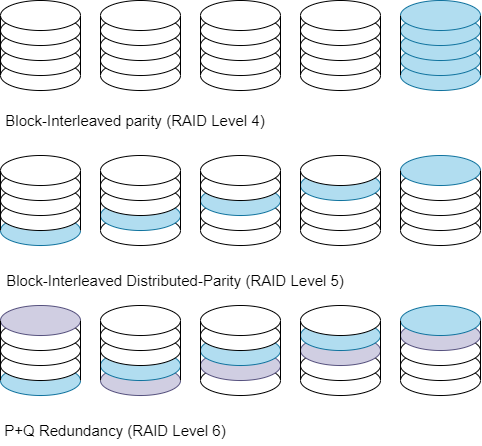
\includegraphics[width=0.9\linewidth]{Images/RAID4-6.drawio.png}
  \caption{RAID levels 4 through 6. The colored platters represent the ones with parity information; white platters contain original data.}
  \label{fig:RAID4-6}
\end{figure}

In this report, we present a RAID-6 based distributed storage system. The rest of the report is organized as follows: Section II presents an overview of the scope of our project. Section III introduces the problem statement of the RAID. Section IV covers the mathematics of the RAID data recovery methods. Section V presents our experiment results with different system configurations. Section VI discusses the scalability of the RAID-6. Section VII concludes our contributions to this project. The mathematics of Galois Field is in Appendix A.

\section{Overview}
The basic function of our RAID-6 based distributed storage system includes:
\begin{itemize}
    \item Store and access abstract “data objects” across storage nodes using RAID-6 for fault-tolerance
    \item Mechanisms to determine the failure of storage nodes
    \item Rebuild of lost redundancy at a replacement storage node
\end{itemize}
We implemented advanced features as follows:
\begin{itemize}
    \item Operation supports different sizes of the data object (data object size compared with the quantum of data of the system)
    \item Adjustable chuck size of the RAID system
    \item Support larger set of configurations (more than 2 checksum disks with an arbitrary number of data disks)
    \item Including the theoretical specification values of the mechanical hard disks to estimate the performance of the real-world operation
\end{itemize}

\section{Problem Statement}
Assuming we have\(\ n \) storage disks as \(\ D_1, D_2, ... D_n\). We prepared\(\ m \) checksum disks for redundancy, \(\ C_1, C_2, ... C_m\). The storage sizes for all\(\ m + n \) disks are the same as \( K \). The goal is to detect the disks that are corrupted and restore up to \(\ m \) disks of either data or checksum.

In RAID-5 and RAID-6, the checksum is distributed into all disks. The number of \(\ m \) represents the number of parities. For RAID-6 setup, \(\ m = 2\). We will be discussing the situations where \(\ m > 2\) in the later sections.

\section{Method}
\subsection{Galois Field}
Galois Field (GF), also known as finite field, defines the mathematical operations for its elements and serves as the mathematical basis of the RAID-6 data recovery mechanism \cite{2007math_of_RAID, 1997Tutorial_Reed, Math_GF}. 

\subsubsection{Prime Field}
Prime field is a basic type of Galois field, which is denoted as $\text{GF}(p)$, where $p$ is a prime number. A prime field $\text{GF}(p)=\{0,1,...,p-1\}$ has the following properties
\begin{itemize}
    \item The result of addition or subtraction of any two of the elements still belongs to $\text{GF}(p)$.
    \item For any three elements $a$, $b$ and $c$, 
    \begin{align}
        &a+b=b+a\\ 
        &(a+b)+c=a+(b+c).
    \end{align}
\end{itemize}
The addition and subtraction are defined as 
\begin{align}
    &\text{add}:(a+b)\text{MOD}(p)\\
    &\text{sub}:(a-b)\text{MOD}(p).
\end{align}
The multiplication and division are defined as 
\begin{align}
    &\text{mul}:(a\cdot b)\text{MOD}(p)\\
    &\text{div}:a/b=(a{{b}^{-1}})\text{MOD}(p),
\end{align}
where $(b\cdot{{b}^{-1}})\text{MOD}(p)=1$.

The reason why $p$ must be a prime number is that the existence of result value within the set is ensured only when $p$ is a prime number, e.g., if $p=4$, there will be no solution when we calculate $(2\times 2^{-1}) MOD(p)=1$.

\subsubsection{Polynomial based on Galois Field}
The Galois field can be applied to the parameters in polynomials. For such polynomials, the parameters belong to the Galois field, and also obey the law of addition, subtraction, multiplication and division operations. 

The addition is calculated by
\begin{align}
  & ({{a}_{0}}+{{a}_{1}}X+...+{{a}_{n}}{{X}^{n}})+({{b}_{0}}+{{b}_{1}}X+...+{{b}_{n}}{{X}^{n}}) \nonumber\\ 
 & =({{a}_{0}}+{{b}_{0}})\text{MOD}(p)+({{a}_{1}}+{{b}_{1}})\text{MOD}(p)X \nonumber\\ 
 & +...+({{a}_{n}}+{{b}_{n}})\text{MOD}(p){{X}^{n}},
\end{align}
and the subtraction can be calculated in the similar way.

The multiplication is calculated by
\begin{align}
  & ({{a}_{0}}+{{a}_{1}}X+...+{{a}_{n}}{{X}^{n}})\times ({{b}_{0}}+{{b}_{1}}X+...+{{b}_{m}}{{X}^{m}}) \nonumber\\ 
 & ={{c}_{0}}+{{c}_{1}}X+...+{{c}_{n+m}}{{X}^{n+m}},
\end{align}
where
\begin{equation}
{{c}_{k}}=\sum\limits_{\begin{smallmatrix} 
 i+j=k, \\ 
 0\le i\le n,0\le j\le m 
\end{smallmatrix}}{{{a}_{i}}\cdot {{b}_{j}}}
\end{equation}


The division is critical to the calculation for the lookup table in the RAID-6 system. For example, if a polynomial belongs to $GF(2)$ is given by 
\begin{align}
    f(X)={{X}^{6}}+{{X}^{5}}+{{X}^{4}},
\end{align}
which is divided by 
\begin{align}
    f(X)={{X}^{4}}+X+1.
\end{align}
The calculation is processed as follows

$$
\begin{array}{lr} 
&X^2+X+1 \\ 
X^4+X+1  \!\!\!\!\!\! & \overline{)X^6 + X^5 + X^4  \text{\ \ \ \ \ \ \ } \text{\ \ \ \ \ \ \ }\text{\ \ \ \ \ \ \ } \text{\ \ \ \ \ \ \ }} \\ 
& \underline{X^6 \text{\ \ \ \ \ \ \ }\text{\ \ \ \ \ \ \ }+X^3+X^2 \text{\ \ \ \ \ \ \ }\text{\ \ \ \ \ \ \ } } \\ 
& {\text{\ \ \ \ \ \ \ } X^5+X^4+X^3+X^2\text{\ \ \ \ \ \ \ }\text{\ \ \ \ \ \ \ }}\\
& \underline{\text{\ \ \ \ \ \ \ } X^5 \text{\ \ \ \ \ \ \ }\text{\ \ \ \ \ \ \ }+X^2+X\text{\ \ \ \ \ \ \ }}\\
&{\text{\ \ \ \ \ \ \ }\text{\ \ \ \ \ \ \ }X^4+X^3\text{\ \ \ \ \ \ \ }+X\text{\ \ \ \ \ \ \ }}\\
&\underline{\text{\ \ \ \ \ \ \ }\text{\ \ \ \ \ \ \ }X^4\text{\ \ \ \ \ \ \ }\text{\ \ \ \ \ \ \ }+X+1}\\
&{\text{\ \ \ \ \ \ \ }\text{\ \ \ \ \ \ \ }\text{\ \ \ \ \ \ \ }X^3+1}
\end{array}
$$

\subsubsection{Extension Field}
The extension field $\text{GF}({{p}^{m}})$ is a mathematical definition derived from the Galois field, whose elements are polynomials based on the Galois field. The parameters in the polynomial belong to $GF(p)$, and the maximum order of $X$ is $m-1$. For example, the parameters in $\text{GF}({{2}^{8}})$ belong to $\text{GF}(2)$, and the polynomial $f(X)={{X}^{8}}$ should be transformed into a polynomial with a maximum order of seven. 

The transformation is conducted by dividing the original polynomials by the corresponding irreducible polynomials. Some irreducible polynomials in $\text{GF}({{2}^{m}})$ is given by
\begin{align}
  & m=4:{{X}^{4}}+X+1 \\ 
 & m=8:{{X}^{8}}+{{X}^{4}}+{{X}^{3}}+{{X}^{2}}+1 \\ 
 & m=16:{{X}^{16}}+{{X}^{12}}+{{X}^{3}}+X+1 
\end{align}

Some transformations in the extension field $GF(2^8)$ are given in Table. \ref{table:GF-2-8}. 

\begin{table*}[htbp]
\caption{Some transformations in $GF(2^8)$} \label{table:GF-2-8}
\begin{center}
\begin{tabular}{c c c c}
\toprule[1pt]
 Original Polynomial            & Transformed Polynomial           & Binary Representation   & Value \\ \hline
  $0$                           & $0$                              & $0000\ 0000$             & $0$      \\
 $X^0$                          & $1$                              & $0000\ 0001$             & $1$      \\
 $X^1$                          & $X$                              & $0000\ 0010$             & $2$     \\
 $X^2$                          & $X^2$                            & $0000\ 0100$             & $4$     \\
 $X^3$                          & $X^3$                            & $0000\ 1000$             & $8$      \\
 $X^4$                          & $X^4$                            & $0001\ 0000$             & $16$      \\
 $X^5$                          & $X^5$                            & $0010\ 0000$             & $32$      \\
 $X^6$                          & $X^6$                            & $0100\ 0000$             & $128$     \\
 $X^7$                          & $X^4+X^3+X^2+1$                  & $0001\ 1101$             & $29$     \\
 $X^8$                          & $X^5+X^4+X^3+X$                  & $0011\ 1010$             & $58$     \\
 $X^9$                          & $X^6+X^5+X^4+X^2$                & $0111\ 0100$             & $116$     \\
\bottomrule[1pt]
\end{tabular}
\end{center}
\end{table*}


Given the extension field $GF(2^8)$ and the corresponding irreducible polynomial (a polynomial that cannot be factored into the product of two non-constant polynomials), the multiplication and division can be accelerated by utilizing the lookup tables $gfilog$ and $gflog$, which are shown in Table. \ref{table:GFlog_GFilog}.

\begin{table}[htbp]
\caption{Some values in the $\emph{gflog}$ and $\emph{gfilog}$ table} \label{table:GFlog_GFilog}
\begin{center}
\begin{tabular}{c c | c c}
\toprule[1pt]
 $gflog$                       & $gfilog$                          & $gflog$                 & $gfilog$ \\ \hline
 $0$                           & $1$                               & $11$                    & $232$      \\
 $1$                           & $2$                               & $12$                    & $205$      \\
 $2$                           & $4$                               & $13$                    & $135$     \\
 $3$                           & $8$                               & $14$                    & $19$     \\
 $4$                           & $16$                              & $15$                    & $38$      \\
 $5$                           & $32$                              & $16$                    & $76$      \\
 $6$                           & $64$                              & $17$                    & $152$      \\
 $7$                           & $128$                             & $18$                    & $45$      \\
 $8$                           & $29$                              & $19$                    & $90$      \\
 $9$                           & $58$                              & $20$                    & $180$      \\
 $10$                          & $116$                             & $21$                    & $117$      \\
\bottomrule[1pt]
\end{tabular}
\end{center}
\end{table}


The $i^{th}$ element in $\emph{gfilog}$ table $\emph{gfilog}[i]$ is the corresponding value of $X^i$ in the extension field, and the table $\emph{gflog}$ is the inverse of $\emph{gfilog}$, i.e., $\emph{gflog}[\emph{gfilog}[i]]=i$. 

The polynomial representation $X^i$ and its numerical value are just different identifiers of the same value in the extension field, so the multiplication of the numerical value is equivalent to the multiplication of its polynomial version. The trick of accelerating multiplication calculation is based on the fact that $X^i\times X^j=X^{i+j}$, i.e., the multiplication can be converted to the addition of the exponent in the polynomial version (Details are given in Appendix A). To calculate $A\otimes B$ ($\otimes$ denotes the XOR operation), we first convert the value to its polynomial version by searching the $\emph{gflog}$ table. Then the result in polynomial representation is given by

\begin{align}
    \emph{gflog} [A]+\emph{gflog} [B].
\end{align}

To obtain the numerical result, we just need to search the $gfilog$ table by taking $gflog[A]+gflog[B]$ as the index.
Thus, the multiplication and division can be calculated by
\begin{align}
  & A\otimes B=gfilog [gflog [A]+gflog [B]] \\ 
 & A\otimes {{B}^{-1}}=gfilog [gflog [A]-gflog [B]].
\end{align}


\subsection{Reed-Solomen Coding}
The original RAID-6 architecture can tolerate only two device crashes. The RS coding is a technique that improves the tolerance of the number of device crashes from two to $n$ in RAID-6 file systems. RS coding is widely used in state-of-art RAID-6 systems and it has been studied and optimized for practical usage in depth. Song et al. \cite{2007RS_1} noticed that real-time constraint of
codec leads to the computational bottleneck of devices. To overcome this bottleneck, they replaced the dominant calculation of the spreading function with small lookup tables and proposed an algorithm to reduce the number of multipliers. Followed by this idea, Trifonov et al. \cite{2015RS_2} utilized cyclotomic fast Fourier transform to reduce the required number of Galois field multiplications for data recovery. 

In this report, we do not dive deep into the complexity reduction of RS coding but only use basic RS coding. 
\subsubsection{Parity Calculation}
The data vector is denoted by $D=[{{d}_{1}},{{d}_{2}},...{{d}_{i}}]$, the parity vector is denoted by $P=[{{p}_{1}},{{p}_{2}},...,{{p}_{i}}]$, and the Vandermonde matrix is given by 
\begin{equation}
   F=\left[ \begin{matrix}
   1 & 1 & ... & 1  \\
   1 & 2 & ... & n  \\
   \vdots  & \vdots  & \ddots  & \vdots   \nonumber\\
   1 & {{2}^{m-1}} & ... & {{n}^{m-1}}  \\
\end{matrix} \right]
\end{equation}

Suppose we have $n$ data disks and $m$ parity disks, to calculate the parity $P_i$, we define function $F_i$ as

\begin{align}
    {{P}_{i}}={{F}_{i}}({{d}_{1}},{{d}_{2}}...,{{d}_{n}})=\sum\limits_{j=1}^{n}{{{d}_{j}}{{f}_{i,j}}},
\end{align}
whose matrix representation is given by 
\begin{align}
    P=FD.
\end{align}
\label{eq:p=fd}

\subsubsection{Data and Parity Recovery}

Define matrix  
$A=\left[ \begin{matrix}
   I  \\
   F  \\
\end{matrix} \right]$ and   
$E=\left[ \begin{matrix}
   D  \\
   P  \\
\end{matrix} \right]$, 
where $I$ is an identity matrix. 
When crashes happen in some disks, we can delete the rows in $A$ and $E$ that are corresponding to the failed disks to obtain
\begin{align}
    {A}'D={E}'.
\end{align}
The original data can be recovered by 
\begin{align}
    D={{{A}'}^{-1}}{E}'.
\end{align}
Once the data is recovered, the parities can be recovered by calculating $P=FD$ again.

\subsection{Further Features}
\subsubsection{Accommodate Real Files of Arbitrary Size}
\begin{figure}[htbp]
  \centering
  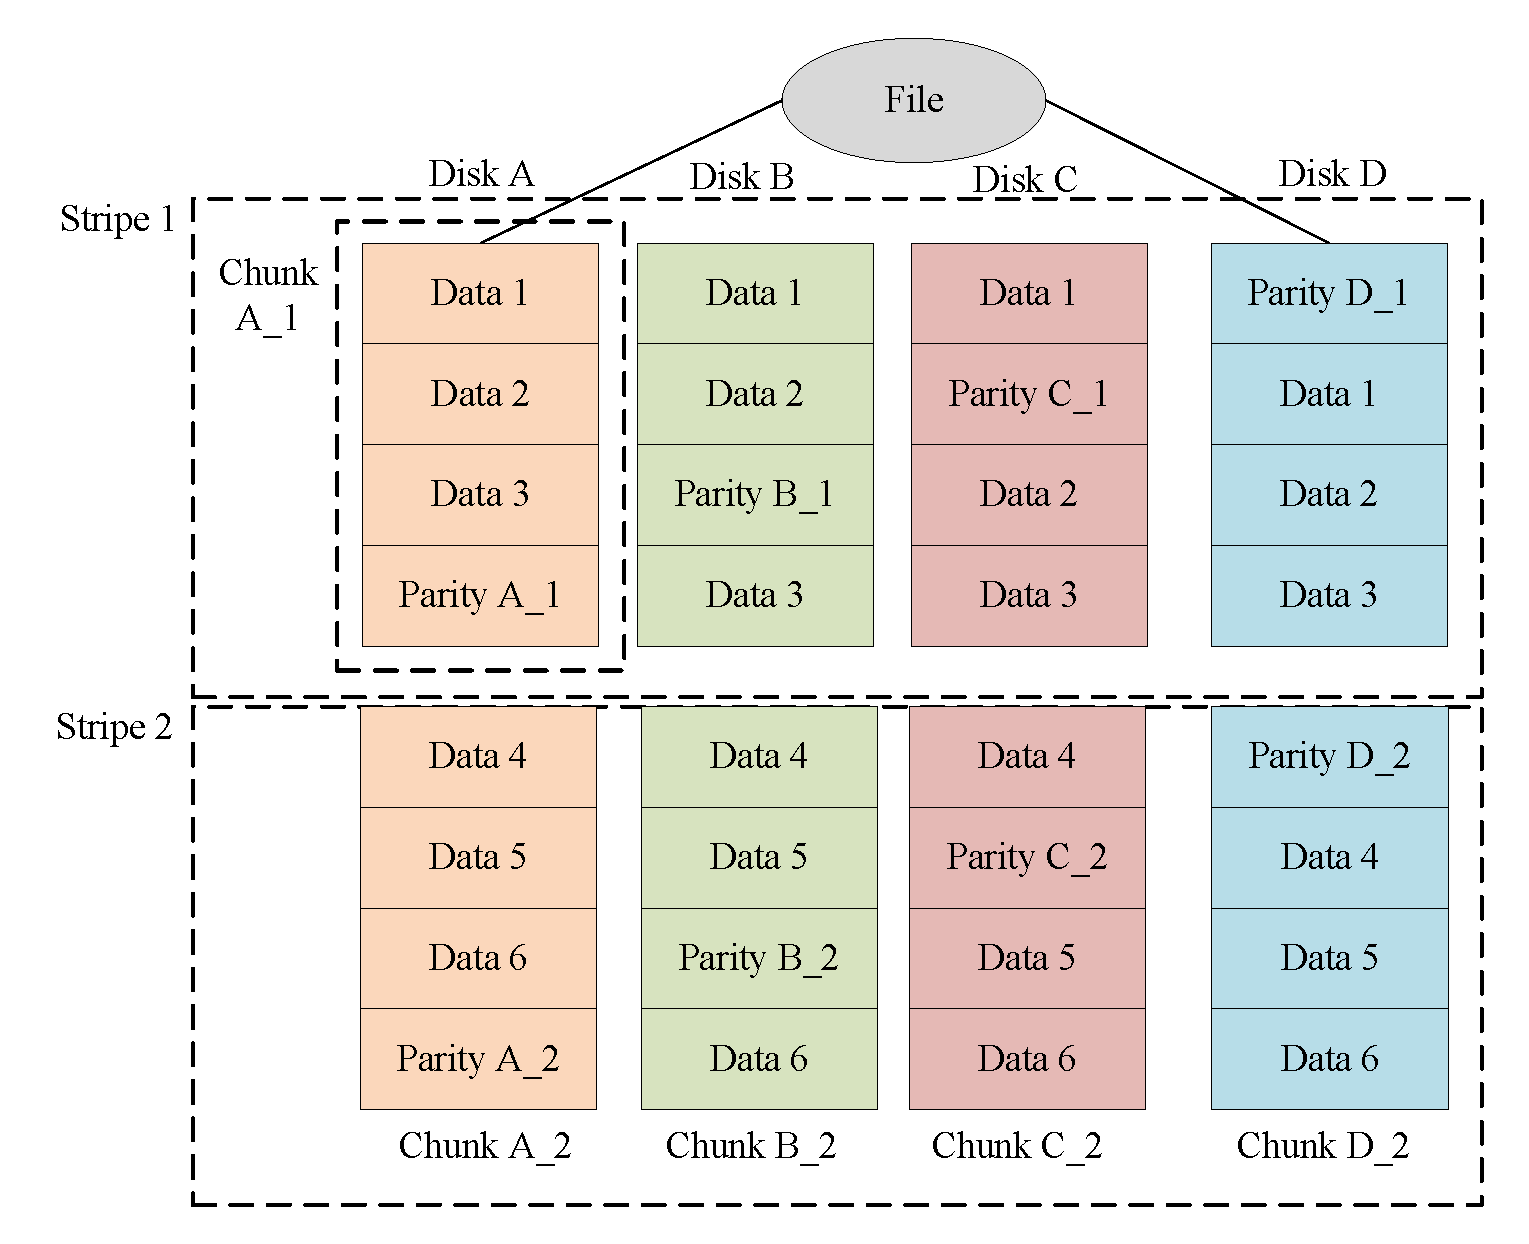
\includegraphics[width=0.9\linewidth]{Images/chunking_model.pdf}
  \caption{Data saving structure.}
  \label{fig:chunking_model}
\end{figure}
In real applications, file sizes vary from several Bytes to x-Mb. It is not reasonable to consider the files as fixed size or calculate the parity according to the entire file. 

The better solution is: to calculate the parity according to fixed-size chunks/strips rather than taking the file as the unit of parity calculation. As shown in Fig. \ref{fig:chunking_model}, the space of each disk is divided into multiple fixed-length chunks, and we take one chunk from each disk to form a stripe. Each stripe is a unit for data storage and parity calculation, i.e., the data within a stripe satisfy all the regulations of Reed-Solomen Coding. A stripe may include an intact file or not, but it does not matter. When we are writing a new file into the disks, it is broken in I/O stream to save the data into any vacant space. After the data writing, all the stripes that are involved update their parities to ensure data consistency. When we want to read a file, we just need to find the physical address of the corresponding data, create an I/O stream, and rebuild the file. For the vacant space, we can initialize them as `0', and update the value when data needs to be stored.

In this way, the influence of file size on the complexity of parity calculation can be significantly reduced. For example, if the number of parity is $M$ and the data size is $N$, the complexity of $P=FD$ is ${\mathrm O}(M{{N}^{2}})$. If we equally divide the data matrix into two matrices, the complexity is reduced to 
\begin{align}
    {\mathrm O}\left( 2M{{\left( \frac{N}{2} \right)}^{2}} \right)={\mathrm O}\left( \frac{1}{2}M{{N}^{2}} \right).
\end{align}

If we take the entire file as a unit, the complexity grows with the increase of file size given by ${\mathrm O}(M{{N}^{2}})$, which is a second-order function of the file size. But if we fix the chunk/stripe size, the complexity according to the file size is given by
\begin{align}
    {\mathrm O}\left( \frac{M{{N}_{f}}}{{{N}_{s}}}{{\left( {{\text{N}}_{s}} \right)}^{2}} \right),
\end{align}
where $N_f$ denotes the file size, and $N_s$ denotes the stripe size (a constant). Given constant $M$ and $N_s$, the complexity is actually a linear function of $N_f$. Thus, it is an efficient way to reduce the complexity of parity calculation by setting a fixed chunk/stripe size.

\subsubsection{Mutable files}
To support mutable files, we take into account updates of the content. When the content of a file is changed, there are three cases:
\begin{itemize}
    \item If the size is not changed, rewrite the space which is occupied by the original file.
    \item If the size is reduced, rewrite the space which is occupied by the original file and release some of the space (mark the corresponding physical address as ``vacant").
    \item If the size is increased, rewrite the space which is occupied by the original file, find more vacant space to save the rest of the data, and record the new physical address.
\end{itemize}

To support the mutable files, the file can be saved at discrete physical addresses, and the disk performance is related to the I/O type and the chunk/stripe size.

\textbf{For read-frequent service} the smaller the chunk/stripe size is, the higher cost of addressing because the file is divided into more pieces. So if the disk is mainly used for read service, a larger chunk/stripe size is better.

\textbf{For write/update-frequent service} smaller chunk/stripe size can reduce the calculation time of parity linearly. But it is not definitely better to set a smaller chunk/stripe size because addressing is also required for writing. So there is a balance between parity calculation and addressing, and the chunk/stripe size needs to be chosen carefully. 

\section{Experiments}
In our experiments, we select Seagate ST4000VM000 as the storage device. The parameters are as follows: 
\begin{itemize}
    \item Average data rate, read/write (MB/s): $146$MB/s
    \item RPM: $5900$
    \item Seek time: $12$ms
    \item Addressing time $=$ seek time $+$ waiting time $= 12+60/5900*1000=22.17$ms
    \item Data stripes: 6
    \item Parities: 2
\end{itemize}

To build a RAID-6 system, multiple hard disks are required to simulate the parallel reading time. Due to the limitation of hardware resources (we do not have that many physical hard disks), we take the theoretical value of read/write rate for our simulation and use the real parity calculation time with the CPU i7-9750H (2.6GHz). Our code is written in Python 3.9, possible optimization of the algorithms/operations is beyond the scope of this report.

\begin{figure}[htbp]
  \centering
  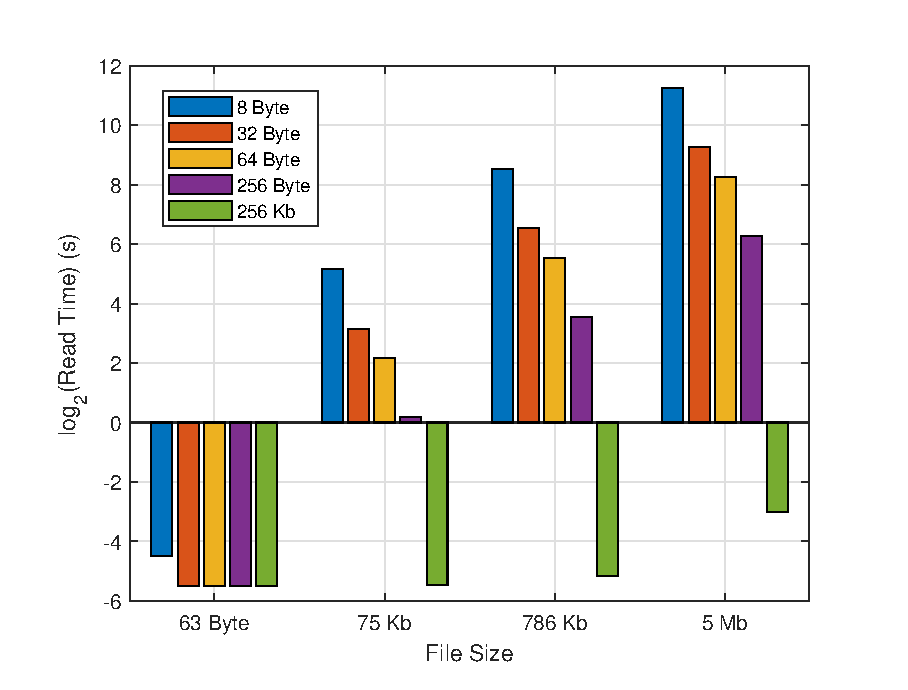
\includegraphics[width=0.9\linewidth]{Images/ReadTime.eps}
  \caption{Reading time under different file sizes and chunk sizes.}
  \label{fig:ReadTime}
\end{figure}
The reading time under different file sizes and chunk sizes is shown in Fig. \ref{fig:ReadTime}. Due to the variant order of magnitudes of different files, we set the $y-$axis as $log_2(time)$. The chunk size is set to $8$ Bytes, $32$ Bytes, $64$ Bytes, $256$ Bytes, and $256$ Kb to show their impact on the reading time. Under $8$ Bytes chunk size (stripe size $48$ Bytes) the system requires more time for the reading service of an extremely small file ($63$ Bytes) than others, because multiple reading loops are needed since $48 < 63$ Bytes. In contrast, the reading time for this file under $32$ Bytes, $64$ Bytes, $256$ Bytes, and $256$ Kb chunk sizes are almost the same, since the file can be stored within a single stripe ($32 \times 6 = 192 > 63$ Bytes) and thus can be read in one loop. Note that the reading time of the disk is small and the addressing time accounts for most of the total time.
When the file size increase from $75$ Kb to $5$ Mb, there is an obvious advantage of larger chunk size over smaller chunk sizes due to less cost of addressing.

\begin{figure}[htbp]
  \centering
  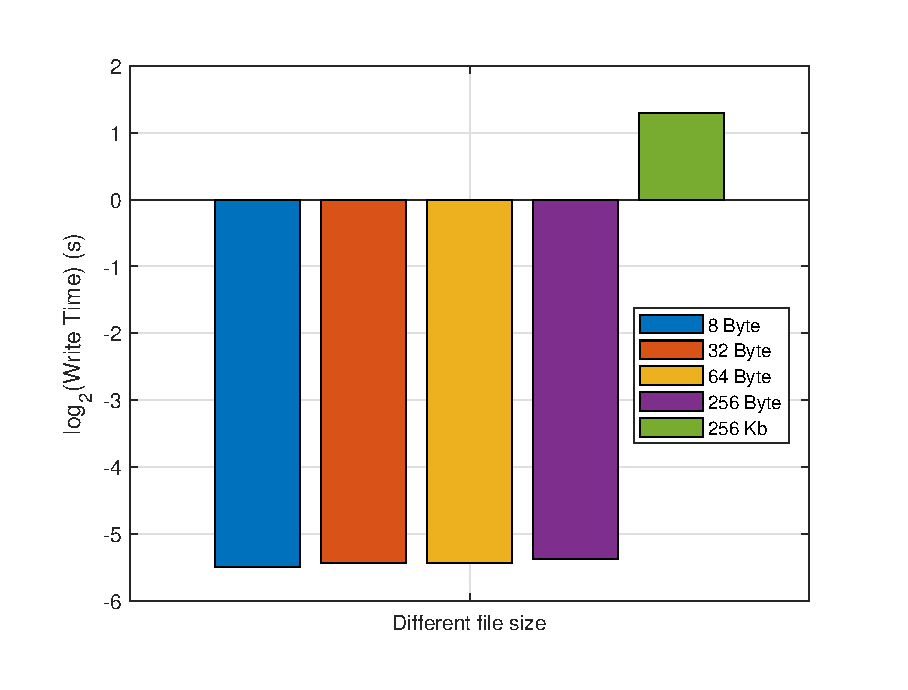
\includegraphics[width=0.9\linewidth]{Images/WriteTime_single.eps}
  \caption{writing time for single stripe under different chunk sizes.}
  \label{fig:WriteTime_single}
\end{figure}
Fig \ref{fig:WriteTime_single} presents the writing time for a single stripe under different chunk sizes. We can find that a larger chunk size requires more time for writing. The difference among the first four chunk sizes is not obvious because the data is reshaped by $log_2$, while it is increasing linearly with the file size.

\begin{figure}[htbp]
  \centering
  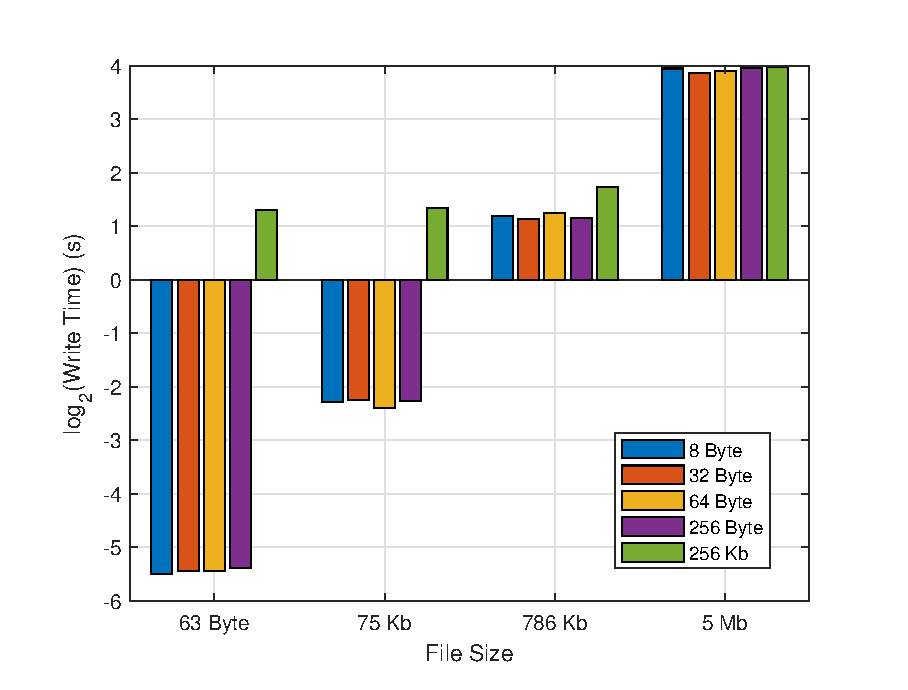
\includegraphics[width=0.9\linewidth]{Images/WriteTime_total.eps}
  \caption{Writing time for the whole file under different chunk sizes and file sizes.}
  \label{fig:WriteTime_total}
\end{figure}
In Fig. \ref{fig:WriteTime_total} we present the writing time for the whole file under different chunk sizes and file sizes. 
We can find that for smaller file sizes, the smaller chunk size is more competitive due to less complexity in parity calculation. 
With the increase in file size, the disadvantage of a larger chunk size ($256$ Kb) is compensated by its advantage in addressing time. The performance reaches a similar value when the file size increases to $5$ Mb. 

\begin{figure}[htbp]
  \centering
  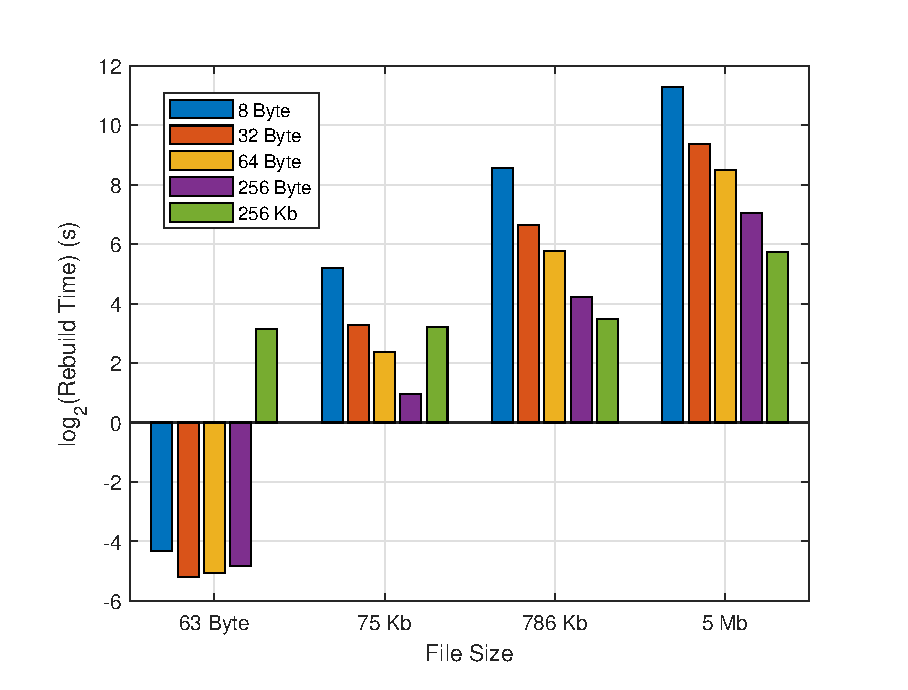
\includegraphics[width=0.9\linewidth]{Images/RebuildTime.eps}
  \caption{Rebuild time under different file sizes and chunk sizes.}
  \label{fig:RebuildTime}
\end{figure}
We also tested the rebuild time for corrupted files as shown in Fig. \ref{fig:RebuildTime}. The advantage of smaller chunk size is less significant than in Fig. \ref{fig:WriteTime_total} because all the involved data are needed for parity calculation when rebuilding a file. But in Fig. \ref{fig:WriteTime_total}, we consider the case that only a small part of the file is changed (only one stripe involved). The tendency in Fig. \ref{fig:RebuildTime} is generally the same, i.e., larger chunk size begins to show its advantage with the increase of file size.

The experiment results indicate that a small chunk size is better for write-frequent services, and a large chunk size is better for read-frequent services. This is in line with the analysis in section IV(C).

\section{Discussion}
% \subsection{Scalability}
In the previous section, we presented the experiment results about chunk size and file size. In this section, we will discuss the possible extension of RAID-6 and the impact on the performance of our proposed method.

Let MTBF (Mean Time Between Failures) denotes the reliability of an individual disk:

\begin{align*}
MTBF_{disk} = \frac{num\ of\ operational\ hours}{num\ of\ failures}
\end{align*}

% The number of disk failures in one group follows the Poisson distribution. 

The failures of disks    are independent events. Once the failure number of disks in a group is larger than \(\ m \), RAID can no longer recover the data.

% \begin{align*}
% P_{RAID\ Failure} = 1 - \sum_{k=0}^{m}{\frac{(MTBF_{disk})^k e^{-MTBF_{disk}}}{k!}}
% \end{align*}

\begin{align*}
MTBF_{Group} = \frac{MTBF_{disk}}{n + m} \times m
\end{align*}

The space utilization of the RAID system can be defined as the number of data disks divided by the total number of disks:

\begin{align*}
Space\ Utilization = \frac{n}{n+m}
\end{align*}

% We discuss the writing efficiency of the RAID system in two situations: one-time operation of a large write, and a large number of scattered small writes. 

In RAID-6, each writing operation requires the disks to read the data, read the first parity, read the second parity... read the \( m^{th}\) parity, write the data, write the first parity, write the second parity... then finally write the \( m^{th}\) parity. We take the performance of writing to a single disk (RAID 0) as the unit for measurement: \( NX\)

For a writing of \( W \) amount of data:
\begin{align*}
Writing\ Performance = \frac{1}{(1+m) \times 2} \times NX
\end{align*}

If we plan to scale the RAID group for more data storage while maintaining the same failure rate, we will have to increase \( m \), the number of checksum disks. The comparison shows in Table \ref{table:Scalability}.


\begin{table} [H]
\caption{RAID Group Scalability Table} \label{table:Scalability}
\begin{center}
\begin{tabular}{c c c c}
\toprule[1pt]
 $n$                            & $6$                               & $12$                      & $24$ \\ \hline
 $m$                            & $2$                               & $4$                       & $8$      \\ \hline
 Space\ Utilization           & $0.75$                            & $0.75$                    & $0.75$      \\
 MTBF                         & $0.25$                            & $0.25$                    & $0.25$      \\
 Writing\ Performance         & $1/6$                             & $1/10$                    & $1/18$     \\
\bottomrule[1pt]
\end{tabular}
\end{center}
\end{table}

Increasing \( m \) at the same ratio as \( n \) does keep the space utilization and failure rate the same, but the writing performance suffers from a larger \( m \). The writing performance decreases at a rate of Logarithm of \( m \). Thus, RAID-6's scalability is not ideal for managing a large number of disks. If a pool of disks needs to be structured as storage with redundancy, they need to be broken into a number of RAID-6 groups where \( m \) of each group is reasonably small. The Galois Field of \(2^{\omega}\) can accommodate \(2^{\omega} - 1\) disks of \(n + m\), when \(\omega = 8\), the 255 disks are enough for one group of RAID-6's usage, there is also no need to use a larger \(\omega\) for larger group size, as that is not desirable from the writing performance standpoint.
 

\section{Conclusion}
We developed a RAID-6 based distributed storage system with features of data storage, parity computation, fault detection, and data rebuilding. We also developed advanced features that provide more freedom in user configuration and generate performance simulation based on the mechanical hard disk's specifications. We discussed the space utilization, fault tolerance, writing performance, and scalability of the RAID-6 system.


% if have a single appendix:
%\appendix[Proof of the Zonklar Equations]
% or
%\appendix  % for no appendix heading
% do not use \section anymore after \appendix, only \section*
% is possibly needed

% use appendices with more than one appendix
% then use \section to start each appendix
% you must declare a \section before using any
% \subsection or using \label (\appendices by itself
% starts a section numbered zero.)
%


\appendices
\section{How Table Gflog and Gfilog accelerate multiplication and division}

Suppose in the extension field GF($2^4$) we are going to calculate \(7 \times 9\). Here the irreducible polynomial is $P(X) = X^4 + X + 1$.

The standard process includes: 1. Transfer the two numbers into a polynomial format. 2. Apply the polynomial multiplication. 3. Check whether the outcome (i.e. the highest power) exceeds the power limit; if so, the outcome is applied to mod ($X^4 + X + 1$): 4. Convert the final outcome from the polynomial format back to the number.

\subsubsection{}
    \begin{align}
        7 &= 0111 = X^2 + X + 1\notag\\ 
        9 &= 1001 = X^3 + 1 \notag
    \end{align}

\subsubsection{}
    \begin{align}
        &7 \times 9\notag\\
        &= (X^2 + X + 1) \times (X^3 + 1)\notag\\
        &= X^5 + X^4 + X^3 + X^2 + X + 1\notag
    \end{align}
\subsubsection{}
    Since the highest power is $5 > (4-1)$, we take the remainder of the result by P(X):
$$
\begin{array}{lr} 
& X+1 \\ 
X^4+X+1 \!\!\!\!\!\! & \overline{)X^5 + X^4 + X^3 + X^2 + X + 1}\\ 
& \underline{X^5 \text{\ \ \ \ \ \ \ }\text{\ \ \ \ \ \ \ \ }+X^2+X \text{\ \ \ \ \ }} \\ 
& {\text{\ \ \ \ \ \ \ } X^4+X^3\text{\ \ \ \ \ \ \ }\text{\ \ \ \ \ \ \ }+1}\\
& \underline{\text{\ \ \ \ \ \ \ } X^4 \text{\ \ \ \ \ \ \ \ }\text{\ \ \ \ \ \ \ \ }+X+1}\\
&{\text{\ \ \ \ \ \ \ \ }\text{\ \ \ \ \ \ \ \ \ }X^3\text{\ \ \ \ \ \ \ \ }+X\text{\ \ \ \ \ }}
\end{array}
$$

\subsubsection{}
    \begin{align}
        &X^3 + X\notag\\
        &= (1010)_{2}\notag\\
        &= (10)_{10}\notag
    \end{align}
Thus, \(7 \times 9 = 10\) in GF($2^4$). \\
    
Note that just like in table \ref{table:GF-2-8}, each number a in GF($2^4$) can be converted to an exponential form $X^m$, where 
    \begin{align}
        a = X^m \ \ \text{MOD} \ \ P(X)
    \end{align}

Now we turn to prove a theorem that will help to do the following transformation:
\newtheorem{thm}{\bf Theorem}
\begin{thm}\label{Thm1}
    Given 
    \begin{align}
        a &= X^m \ \ \text{MOD} \ \ P(X)\\
        b &= X^n \ \ \text{MOD} \ \ P(X)
    \end{align}
    Then in the extension Field:
    \begin{align}
        a \times b = X^{m+n} \ \ \text{MOD} \ \ P(X)
    \end{align}
\end{thm}

The proof is simple and as follows:

\begin{proof}
By integer division and definition, there must be integers $i$ and $j$ satisfying that: 
    \begin{align}
        P(X) \times i + a &= X^m\\
        P(X) \times j + b &= X^n
    \end{align}
Thus, \(a \times b =\)
    \begin{align}
        (X^m - P(X) \times i)(X^n - P(X) \times j) \ \ mod \ \ P(X) \\
        = [X^{m+n} - X^m \times P(X) \times j - X^n \times P(X) \times i \notag \\
        + P(X)^2 \times i \times j] \ \ mod \ \ P(X) \\
        = X^{m+n} \ \ mod \ \ P(X)
    \end{align}
Since in (30) the last three items all include P(X), they are all divisible by P(X). Therefore, only the first item $X^{m+n}$ is left, and the proof is done.
\end{proof}

By Theorem \ref{Thm1}, we see a brand new method of computing multiplication in GF($2^4$) which requires almost no polynomial computation: to compute $a \times b$, just find their corresponding transformation form of $X^m$ and $X^n$, then we re-convert $X^{m+n}$ to the form in the extension field and get the outcome. The first transformation from $a/b$ to the $x^m$ or $x^n$ is done by table $gflog$ and the second which converts $x^{m+n}$ to the number in the extension field is done by table $gfilog$. Note that the exponent $m+n$ might exceed the limit $2^4 = 16$ and requires $mod \ \ 2^4 - 1$ first.

For example, compute \(7 \times 9\) in GF($2^4$) again given that in the table $gflog[7] = 10$ (which denotes $7 = 2^{10} \ \ mod \ \ P(X)$), $gflog[9]=14$ and $gfilog[9] = 10$ (which denotes $10 = 2^9 \ \ mod \ \ P(X)$):
    \begin{align}
        &7 \times 9\notag\\
        &= 2^{10 + 14} \ \ \text{MOD} \ \ P(X)\notag\\
        &= 2^{24}\ \ \text{MOD} \ \ P(X)\notag\\
        &= 2^{9}\ \ \text{MOD} \ \ P(X)\notag\\
        &= 10\notag
    \end{align}
The new multiplication is done only by checking tables (remember that these tables can be calculated in advance) and mod $2^4 -1$ if necessary, which is much more convenient.

The division operation is similar to multiplication as long as the $b^{-1}$ is calculated in advance.

\ifCLASSOPTIONcaptionsoff
  \newpage
\fi



% trigger a \newpage just before the given reference
% number - used to balance the columns on the last page
% adjust value as needed - may need to be readjusted if
% the document is modified later
%\IEEEtriggeratref{8}
% The "triggered" command can be changed if desired:
%\IEEEtriggercmd{\enlargethispage{-5in}}

% references section

% can use a bibliography generated by BibTeX as a .bbl file
% BibTeX documentation can be easily obtained at:
% http://mirror.ctan.org/biblio/bibtex/contrib/doc/
% The IEEEtran BibTeX style support page is at:
% http://www.michaelshell.org/tex/ieeetran/bibtex/
%\bibliographystyle{IEEEtran}
% argument is your BibTeX string definitions and bibliography database(s)
%\bibliography{IEEEabrv,../bib/paper}
%
% <OR> manually copy in the resultant .bbl file
% set second argument of \begin to the number of references
% (used to reserve space for the reference number labels box)
% \begin{thebibliography}{1}

% \bibitem{IEEEhowto:kopka}


% \end{thebibliography}

\bibliographystyle{ieee}
\bibliography{ref}

% biography section
% 
% If you have an EPS/PDF photo (graphicx package needed) extra braces are
% needed around the contents of the optional argument to biography to prevent
% the LaTeX parser from getting confused when it sees the complicated
% \includegraphics command within an optional argument. (You could create
% your own custom macro containing the \includegraphics command to make things
% simpler here.)
%\begin{IEEEbiography}[{\includegraphics[width=1in,height=1.25in,clip,keepaspectratio]{mshell}}]{The rest of the report is organized as follows:}
% or if you just want to reserve a space for a photo:

% \begin{IEEEbiography}{Michael Shell}
% Biography text here.
% \end{IEEEbiography}

% % if you will not have a photo at all:
% \begin{IEEEbiographynophoto}{John Doe}
% Biography text here.
% \end{IEEEbiographynophoto}

% % insert where needed to balance the two columns on the last page with
% % biographies
% %\newpage

% \begin{IEEEbiographynophoto}{Jane Doe}
% Biography text here.
% \end{IEEEbiographynophoto}

% You can push biographies down or up by placing
% a \vfill before or after them. The appropriate
% use of \vfill depends on what kind of text is
% on the last page and whether or not the columns
% are being equalized.

%\vfill

% Can be used to pull up biographies so that the bottom of the last one
% is flush with the other column.
%\enlargethispage{-5in}



% that's all folks
\end{document}


